\documentclass[12pt]{extarticle}
\usepackage[T2A]{fontenc}
\usepackage[utf8]{inputenc}
\usepackage[english, russian]{babel}
\usepackage[a4paper, portrait, margin=2.4cm]{geometry}
\usepackage{mathastext}
\usepackage{amsmath}
\usepackage{amssymb}
\usepackage{graphicx}
\usepackage{multirow}
\usepackage{ragged2e}
\usepackage{wrapfig}
\pagenumbering{arabic}
\graphicspath{{/}}
\newcommand\tab[1][1cm]{\hspace*{#1}}

\begin{document}

\section*{6}
\[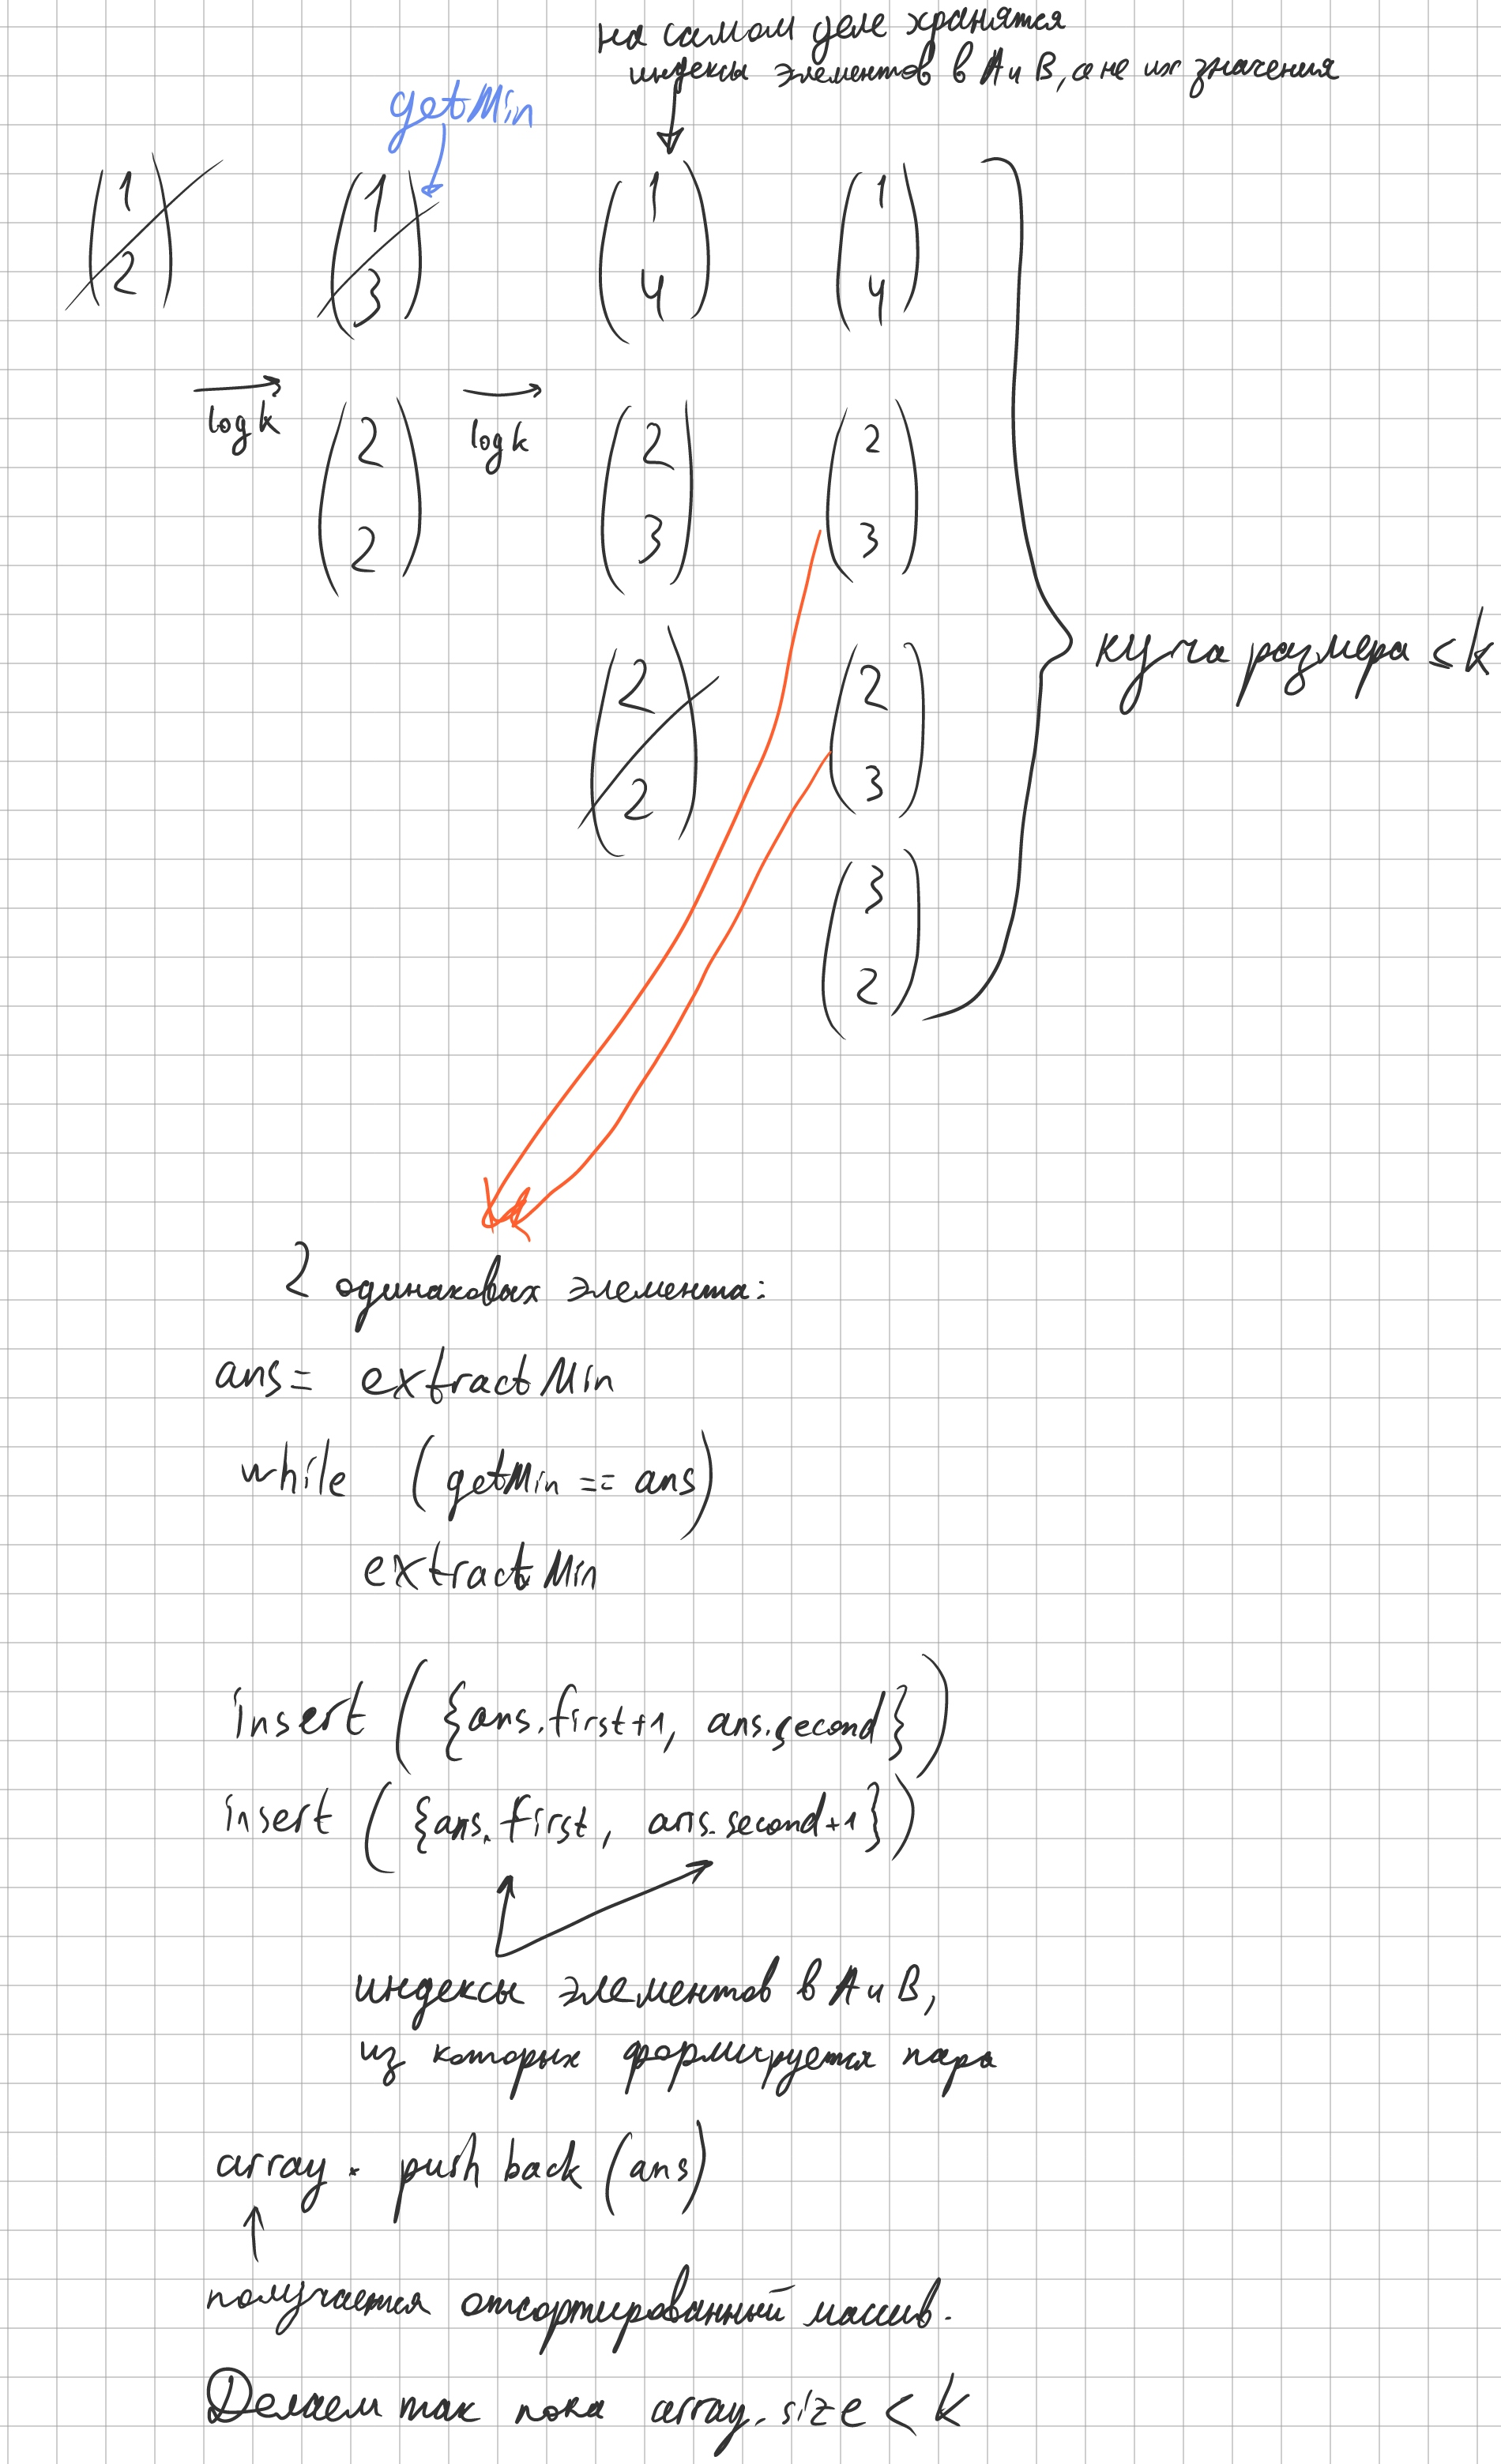
\includegraphics[width=13cm]{6.jpg}\]

\section*{5}
Делаем обычную кучу на минимум, в добавок к которой будем хранить значение наибольшего элемента в ней.
Insert, getMin и extractMin работают за O(logn).
Insert может обновить наибольший элемент (сравнение и обновление - O(1)). ExtractMin обновляет наибольший элемент только если к моменту вызова extractMin в куче оставался только один элемент (после его удаления maxElement = $-\infty$). Поэтому обновлений почти не будет. GetMax работает за O(1).

\section*{3}
Для каждой клетки v[i][j] (если она 0) считем расстояние h до ближайшей единицы сверху. h[i][j] = h[i-1][j] + 1. Если сверху нет ни одной единицы, то это расстояние до границы матрицы. Подсчёт такого расстояния за O(1). Значит подсчёт всего h за n*n.

Считаем максимальное количество подряд идущих клеток в строке i слева от v[i][j] таких, что h для них $\ge$ h[i][j]. Запишем это значение в массив l[][]. Для этого для каждой строчки матрицы создаём стэк s. l[i][0] = 0; s.push({h[i][0], 0}). Для каждого j: удаляем элементы из s пока s.top().first $\ge$ h[i][j]. l[i][j] = j - s.top().second; s.push({h[i][j], j}). Для каждой строки создаётся один стэк, на каждую строку тратится n времени. Значит подсчёт всего l за n*n.

Аналогично считаем массив r[][] для количества подряд идущих клеток в строке i справа от v[i][j]. Надо будет проходиться от v[i][n - 1] до v[i][0].

Проходимся по матрице за n*n и считаем площади всех возможных максимальных прямоугольников и обновляем на каждом шаге ответ. Area[i][j] = h[i][j] * (l[i][j] + r[i][j] + 1); Ans = max(area)

Время работы 4*n*n = O(n*n)

\section*{9}
Проходимся по массиву a[] и для каждого i делаем swap(a[i], a[a[i]]) пока i не станет равен a[i], но не более a.size() раз. Потом проходимся второй раз и смотрим на равенство i и a[i]. Если не равно, то a[i] встречается больше одного раза.

Пусть для какого-то i было сделано k swap. Тогда после этого k элементов стоят на нужных местах (a[j] = j). Для этих k элементов swap не будет вызван ни разу. Значит всего будет сделано не более n перестановок, и асимптотика O(n). Дополнительный массив не создаётся, всё меняется в исходном, поэтому памяти тратится O(1).

\section*{10}
\subsection*{Сортировка слиянием}
Предположим что есть две стабильно отсортированные половины. При слиянии будем класть в полный отсортированный массив первый элемент из первой половины, если он меньше или равен первому элементу из второй. Тогда если будут встречены два равных элемента, то сначала положится тот, который был в первой половине. Значит полный массив будет отсортирован тоже стабильно. По индукции получается, что сортировка слиянием - стабильна.

\subsection*{Быстрая сортировка}
В классической реализации индексы с двух сторон изменяются до тех пор, пока a[i] != pivot. То есть может получиться, что a[i] == a[j] == pivot и они поменяются местами. То есть быстрая сортировка не стабильна.

Её можно сделать стабильной, если хранить не значения элемнтов, а пары (значение, индекс в исходоном массиве). Тогда не будет случаев, когда 2 элемента равны, и не будет перестановок, приводящих к нестабильности.


\section*{4}
Когда делается детерменированный поиск порядковой статистики, на каждом шаге массив разбивается примерно пополам, и в левой половине все элементы оказываются $\le$ элемментов в правой половине. Перестановка элементов в двух половинах занимает много времени. Можно хранить в массиве b пары {left, right}, которые означают, что элементы a[left:middle] меньше или равны a[middle + 1, right]. Тогда если на каком-то шаге надо рассмотреть отрезок [left:right], а он уже есть в b, то можно не тратить время на его почти сортировку.

\section*{1}
Так как менять местами можно только соседние элементы, то если элемент поучаствовал в чётном количестве перестановок, он не поменял чётность своей позиции в массиве.

Создадим массив пар (значние, индекс в исходном массиве). Отсортируем его за O(nlogn). Проходимся по нему; пусть рассмотриваемый элемент равен x. Найдём за O(logn) индексы в отсортированном массиве первого и последнего элементов, равных x. Пусть есть k элементов, равных x. За O(1) можно посчитать, сколько должно быть элементов равных x с чётными и нечётными индексами, за O(k) можно проверить, сколько таких есть. Если значния не совпадают, то ответ на задачу - нет. После этого будем рассматривать элемент, больший x. Правая граница x уже найдена, поэтому переход будет за O(1). $\sum k = n$, значит проверка всех элементов будет за O(nlogn). 

\section*{2}
Сделаем LSD, но сортировать будем не по одной цифре, а по стольким, что $10^m \ge \sqrt{k}$. m - количество цифр, m минимально. Тогда каждая сортировка подсчётом будет работать за O(n + $10^m$) = O(n + $\sqrt{k}$). В таком случае будет сделано всего 2 сортировки подсчётом, потому что если $10^m \ge \sqrt{k}$, то $10^{2m} \ge k$. k - максимальное число в массиве.



\end{document}